\chapter{Introduction}

Wikipedia defines gamification as ``the use of game play mechanics for non-game applications, particularly consumer-oriented web and mobile sites, in order to encourage people to adopt the applications'' \cite {Wikipedia}. \\

The term gamification only came into widespread use in February 2010, as part of the DICE 2010 conference. Jesse Schell, a game designer and professor from Carnegie Mellon, gave a presentation entitled ``the future of games'' in which he claimed that elements of games will invade every part of our daily lives \cite {schell2010design}. The term gained more prominence through several recent books such as Gabe Zichermann's "Game Based Marketing" \cite {zichermann2010game}, who advocated the use of game mechanics in marketing, and Jane McGonigal's "Reality is Broken" \cite {mcgonigal2011reality}, who claimed  that games will make us better human and game is a solution to the broken reality. Finally, Baron Reeves's ``Total Engagement'' \cite {reeves2009total}, who claims that games and virtual worlds will change the way people work and businesses compete. At SXSW 2011, entrepreneur Seth Priebatsch talks about games as the new layer that similar to the social layer, "will change the world" \cite {Priebatsch2010ted}. \\

In IT industry research, Gartner predicts that by 2015, more than half of companies managing innovation processes will employ gamification, a process of applying game mechanics to non-game contexts \cite {gartnerPress2011}. In that same time frame, M2 Research forecasts that game mechanics production will generate \$1.6 billion in revenues and will account for 23\% of social media marketing budgets \cite {M2Research2011}. As of today, existing gamified applications already range across diverse application areas in including productivity, finance, health, sustainability, news, user-generated content and e-learning. Several vendors, mainly startups, offer gamification as a service layer of reward and reputation systems with points, badges, levels and leader boards, with a recent spate of venture capital investment in this emerging industry.\\

In the 2011 Gartner Hype Cycle report, gamification, along with big data and the internet of things, are new additions \cite {gartnerPress2011HypeCycle}. According to Gartner, gamification is on the rise to the peak of the hype, the stage of the "peak of inflated expectation", with a subsequent 5-10 years required for mainstream adoption, as shown in figure 1.1. 
Gartner uses hype cycle theory to track technology adoption: after the peak period, the technology will slip into the trough of disillusionment, after which some technologies will start climbing the slope of enlightenment and eventually reach the plateau of productivity.  As with any technology, gamification will inevitably slip into the disillusionment trough where the hype is passed and the masses realize that there are a lot of unsolved problems. The question remains if gamification will eventually climb out of the trough and appear in the plateau of the cycle.

\begin{figure}[htbp]
	\centering
		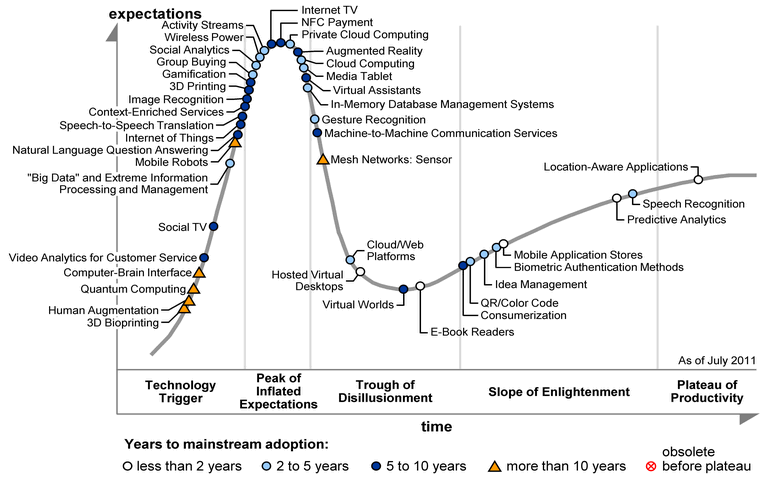
\includegraphics[scale=0.55]{gartner-hype-cycle-2011.png}
		\caption{2011 Gartner Hype Cycle (source: Gartner) \cite {gartnerPress2011HypeCycle}}
		\label{fig:Gartner-2011-Hype-Cycle}
\end{figure}

In fact, there is already quite a lot criticism of gamification in the media. Some call it a mere buzzword, a hyped-up version of a mileage loyalty program, or a superficial ``pointification'', which often misses elements such as storytelling and experiences which are central to what make games effective  \cite {robertson2010}. More and more game designers and researchers are looking into the deeper practice of gamification. Amy Jo Kim presents ``Smart Gamification'' which focuses on designing an effective ``Player Journey'' with intrinsic rewards preferred over extrinsic rewards \cite {Kim2010}. Jane Mcgonigal emphasizes the aspect of ``Playfulness'' in gamification instead of game mechanics \cite {mcgonigal2011}. Similarly, researcher Sebastian Deterding criticizes the current practice of simplistic gamification and stresses the importance of ``meaningful play'' in his Google Tech Talk ``Getting Gamification Right'' \cite {Deterding2011meaningful}.\\

As the preceding shows, Gamification is quickly becoming an IT phenomenon, with some argue it is a meaningless buzzword, while other argue it will revolutionize information technology in the same way as social networks.\\

The goal of this document is to review the different gamification design thoughts and approaches as thoroughly as possible, and to examine commonly employed game mechanics with respect to their usage and effectiveness. In order to provide quantitative insight into the research in gamification, we will also examine the gamification metrics of gamified applications.
